\chapter{Background}
\label{Background}
\section{RoboCup}
The RoboCup competition was initially inspired by Hiroaki Kitano~\cite{robocup} in 1993 and his idea eventually led to the establishment of the RoboCup Federation. The RoboCup competition has a bold vision: ``By the year 2050, to develop a team of fully autonomous humanoid robots that can win against the human world soccer champions''. All the teams participating in RoboCup have to find real-time solutions to some of the most difficult problems in robotics (perception, cognition, action, coordination). All the divisions in RoboCup (soccer, RoboCup@Home, RoboRescue, etc.) are designed so as to test the proposed solutions by the various teams to the problems mentioned above. So far, the researchers participating in RoboCup have made a lot of progress in solving real-world problems that show up in the various RoboCup leagues within each division.

\subsection{Standard Platform League}
The Standard Platform League (SPL) is one of the many leagues in the soccer division of RoboCup. In this league all the teams use the same robot, the Aldebaran NAO humanoid robot, and they focus only on algorithm design and software development for this robot. For this reason, the teams are prohibited to make any changes to the hardware of the robot. The robots are completely autonomous and no human intervention from team members is allowed during the games. The only interaction of the robots with the ``outer world'' is the reception of data from the Game Controller, a computer that broadcasts information about the state of the game (score, time, penalties, etc.).

\begin{figure}[t!]
	\begin{center}
		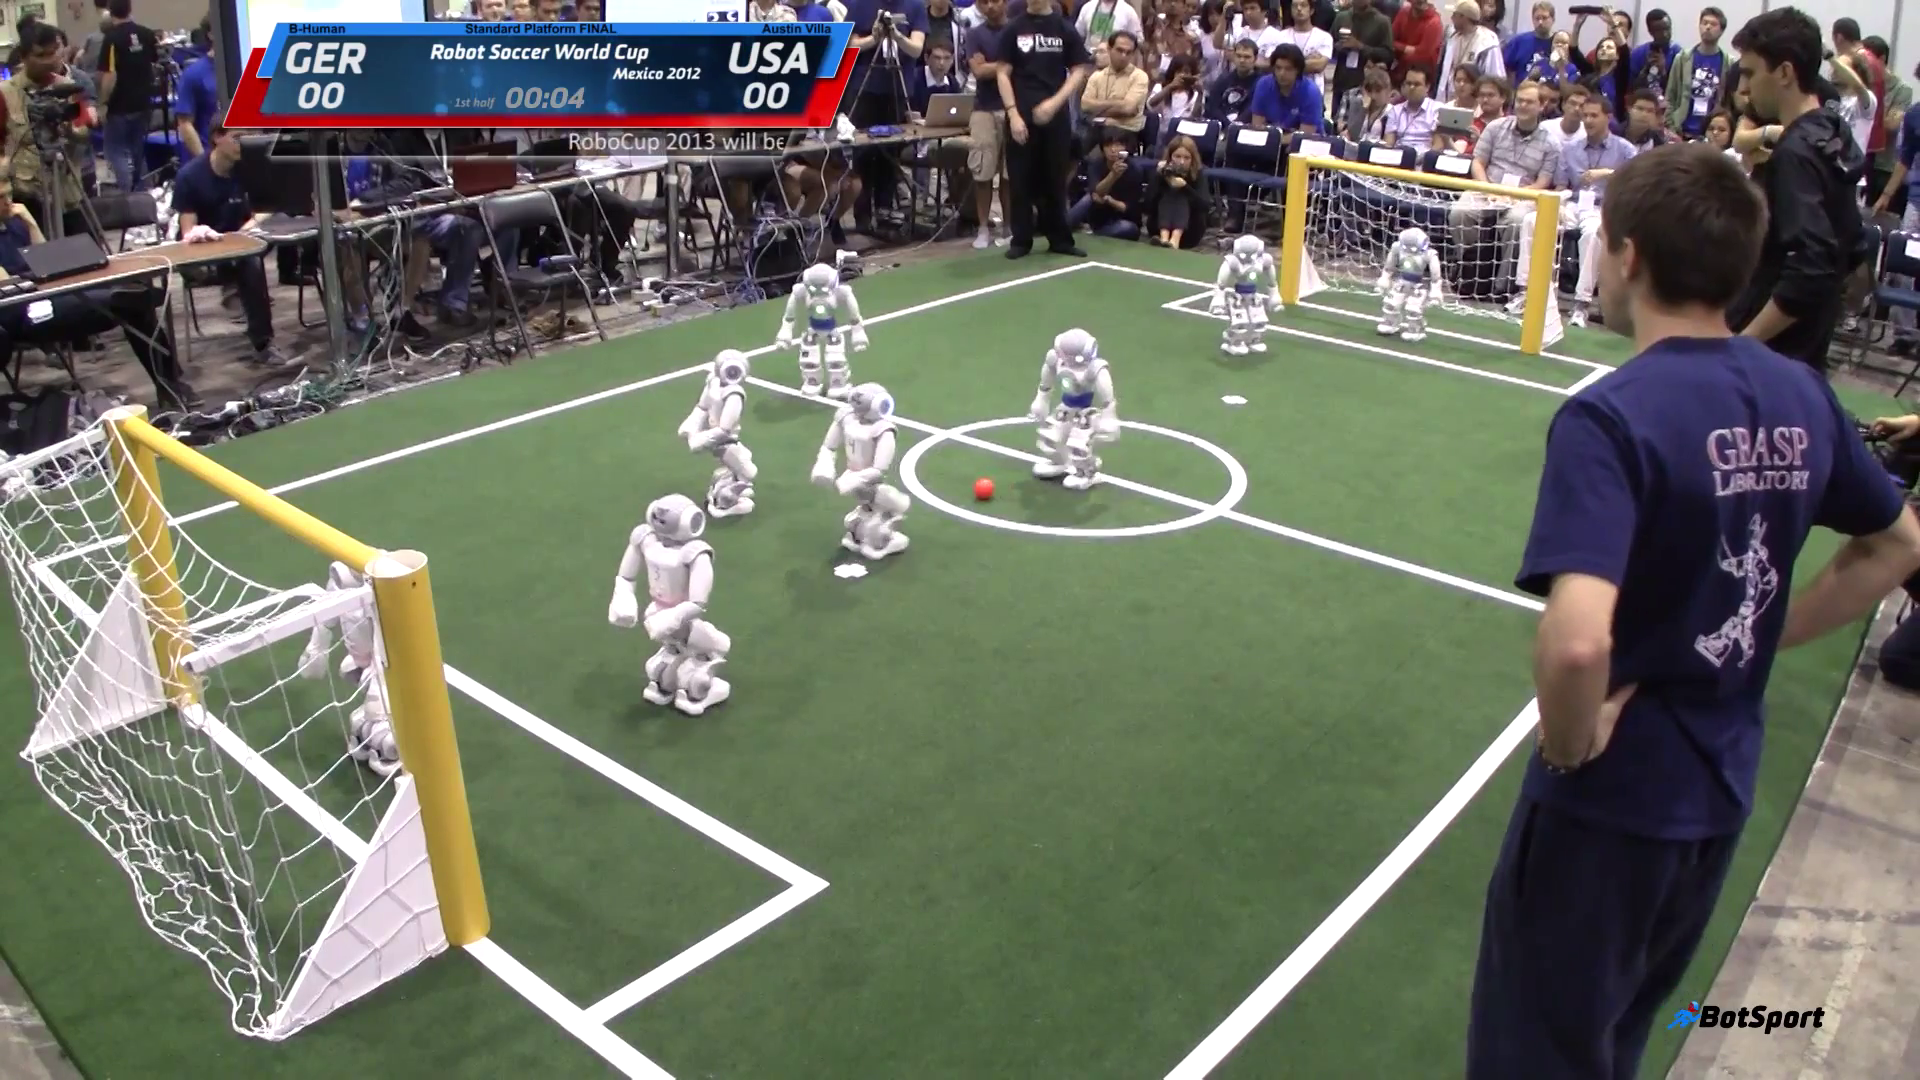
\includegraphics[width=.9\textwidth]{Figures/spl2012.png}
 		\caption{Standard Platform League at RoboCup 2012 (from \url{www.botsport.tv})}
 		\label{fig:RoboCup SPL}
	\end{center}
\end{figure}

Currently, the SPL games are conducted on a field with dimensions $4m \times 6m$~\cite{SPLrules2012}. The field consists of a green carpet marked with white lines and two yellow goals (Figure~\ref{fig:RoboCup SPL}). The appearance of the field is similar to a real soccer field, but it is scaled to the size of the robots. The ball is an orange street hockey ball. Each team consists of four robots and each robot carries a colored waist band (blue or pink) that distinguishes the teams. The total game time is 20 minutes and is broken in two halves; each half lasts 10 minutes.




\begin{figure}[t!]
	\begin{center}
		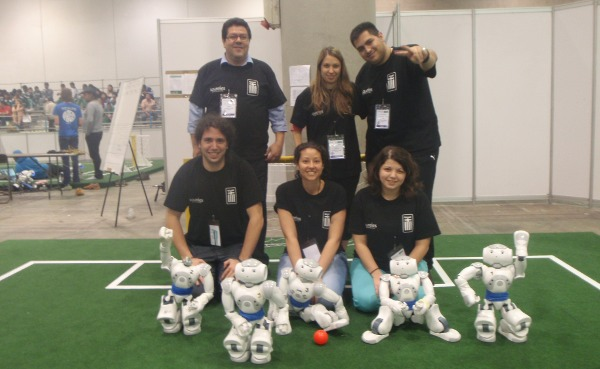
\includegraphics[width=.9\textwidth]{Figures/robocup2012-team.jpg}
 		\caption{Team Kouretes at RoboCup 2012 in Mexico City}
 		\label{fig:Kouretes2012}
	\end{center}
\end{figure}

\section{Robocup SPL Team Kouretes}

Team Kouretes (\url{www.kouretes.gr}) is the RoboCup team of the Technical University of Crete. The team was founded in 2006 and participates in the main RoboCup competition ever since in various leagues (Four-Legged, Standard Platform, MSRS, Webots), as well as in various local RoboCup events (German Open, Mediterranean Open, Iran Open, RC4EW, RomeCup) and RoboCup exhibitions (Athens Digital Week, Micropolis, Schoolfest). In May 2010, the team hosted the 1st official SPL tournament in Greece (with three invited teams) within the Hellenic Conference on Artificial Intelligence (SETN). Distinctions of the team include: {\bf 2nd} place in MSRS at RoboCup 2007; {\bf 3rd} place in SPL-Nao, {\bf 1st} place in SPL-MSRS, among the {\bf top 8} teams in SPL-Webots at RoboCup 2008; {\bf 1st} place in RomeCup 2009; {\bf 6th} place in SPL-Webots at RoboCup 2009; {\bf 2nd} place in SPL at RC4EW 2010; and {\bf 2nd} place in SPL Open Challenge Competition at RoboCup 2011 (joint team Noxious-Kouretes).

The team has been developing its own (publicly-available) software for the Nao robots since 2008. The team code repository includes a custom software architecture, a custom communication framework, graphical tools for monitoring and behavior specification, and modules for object recognition, state estimation, localization, obstacle avoidance, behavior execution, team coordination. The members of the team are senior undergraduate ECE students working on their diploma thesis on a RoboCup-related topic; 15 diploma theses have been completed so far. Recently, the team participated in the RoboCup German Open 2012 competition in Magdeburg, in RoboCup Iran Open 2012 in Tehran, and in RoboCup 2012 in Mexico City (Figure~\ref{fig:Kouretes2012}). In the most recent RoboCup 2012 competition, the team succeeded to proceed to the second round-robin round and rank among the top-16 SPL teams in the world.

\section{Aldebaran NAO Humanoid Robot}
NAO is an integrated, programmable, medium-sized humanoid robot developed by Aldebaran Robotics in Paris, France~\cite{naopaper}. Project NAO started in 2004. In August 2007 NAO officially replaced Sony's AIBO quadruped robot in the RoboCup SPL. In the past few years NAO has evolved over several designs and several versions. 

\begin{figure}[t!]
	\begin{center}
		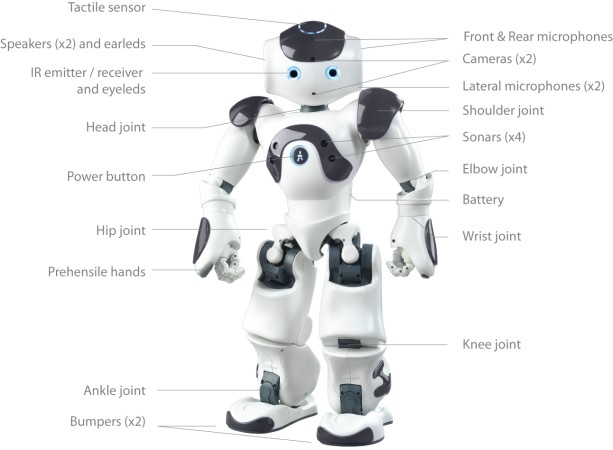
\includegraphics[height = 8cm]{Figures/nao.jpg}
 		\caption{Components of NAO v3.3}
 		\label{fig:sensors}
	\end{center}
\end{figure}

NAO (version V3.3) is a 58cm, 5kg humanoid robot (Figure~\ref{fig:sensors}). The NAO robot carries a fully capable computer on-board with an x86 AMD Geode processor at 500 MHz, 256 MB SDRAM, and 2 GB flash memory running an Embedded Linux distribution. It is powered by a 6-cell Lithium-Ion battery which provides about 30 minutes of continuous operation and communicates with remote computers via an IEEE 802.11g wireless or a wired ethernet link. 

NAO RoboCup edition has 21 degrees of freedom; 2 in the head, 4 in each arm, 5 in each leg and 1 in the pelvis (there are two pelvis joints which are coupled together on one servo and cannot move independently). NAO, also, features a variety of sensors. Two cameras are mounted on the head in vertical alignment providing non-overlapping views of the lower and distant frontal areas, but only one is active each time and the view can be switched from one to the other almost instantaneously. Each camera is a $640 \times 480$ VGA devise operating at 30fps. Four sonars (two emitters and two receivers) on the chest allow NAO to sense obstacles in front of it. In addition, the NAO has a rich inertial unit, with one 2-axis gyroscope and one 3-axis accelerometer, in the torso that provides real-time information about its instantaneous body movements. Two bumpers located at the tip of each foot are simple ON/OFF switches and can provide information on collisions of the feet with obstacles. Finally, an array of force sensitive resistors on each foot delivers feedback of the forces applied to the feet, while encoders on all servos record the actual values of all joints at each time.



\section{Robot Kinematics}
A \textit{robot kinematic chain} is an articulated manipulator that interacts with the environment and is typically described as an assembly of robotic links connected by (rotary) joints. The joints rotate and control the relative angular positioning of the links of the manipulator. Not all combinations of joints' positions in the chain are valid, because some combinations lead to collisions between the links of the chain or with some fixed item of the environment, such as the floor or a wall. All the valid combinations of joint values form the \textit{joint space}. The term \textit{degrees of freedom} (DOF) refers to the number of joints in a kinematic chain; clearly, more DOF imply more flexibility in the motion of the chain. 

\textit{Robot kinematics} is the application of geometry to the study of  kinematic chains with multiple degrees of freedom. More specifically, robot kinematics provide the transformation from the joint space, where the kinematic chains are defined, to the Cartesian space, where the robot manipulator moves, and vice versa. Robot kinematics are quite useful, because they can be used for planning and executing movements, as well as calculating actuator forces and torques.



\subsection{Forward Kinematics}
The joint space reveals very little information about the position and orientation of the end effector of the kinematic chain. The \textit{forward kinematics} define a mapping from the joint space to the three-dimensional Cartesian space. Given a kinematic chain with $m$ joints and a set of joint values $(\theta_1, \theta_2,\ldots,\theta_m)$, the forward kinematics can find the position $(p_x,p_y,p_z)$ and the orientation $(a_x,a_y,a_z)$ of the end effector of the kinematic chain in the three-dimensional $x$-$y$-$z$ space. Forward kinematics is a domain-independent problem and can be solved for any simple or complex kinematic chain yielding a closed-form, analytical solution. 

\subsection{Inverse Kinematics}
Robot manipulators typically need to reach target points or follow trajectories in the three-dimensional space. To make the end effector reach a point or follow a trajectory, one has to specify appropriate values for the joints of the kinematic chain. The \textit{inverse kinematics} define ways to go from the three-dimensional space to the joint space. In particular, the inverse kinematics define a relation between points in the three-dimensional space (position $(p_x,p_y,p_z)$ and orientation $(a_x,a_y,a_z)$) and joint values/angles $(\theta_1, \theta_2,\ldots,\theta_m)$ in the joint space of a kinematic chain with $m$ joints. The problem of inverse kinematics is domain-dependent and every kinematic chain has a different solution. The solution to the inverse kinematics problem can lead to an analytical, closed-form equation or to a numerical, iterative approximation (e.g. with the Jacobian approximation method). As the number of DOF increases, a point in the three-dimensional space may have more than one matching points in the joint space. This multiplicity of solutions makes the inverse kinematics a relation, not a mapping.




\section{Affine Transformations}
An affine transformation is a mapping that transforms points and vectors from one space to another, in a way that preserves the ratios of distances. The source and target spaces can be $n$-dimensional with $n\ge2$. The following are affine transformations: geometric contraction, expansion, dilation, reflection, rotation, shear, similarity transformations, spiral similarities, and translation. All the possible combinations of the above produce an affine transformation as well. The flexibility of affine transformations with respect to object representation in different spaces, makes it a very useful tool in computer graphics.

For the purposes of this thesis we only use rotation and translation, so we will focus only on these two types of affine transformation. Additionally, we are working in a three-dimensional Cartesian work space and therefore all the definitions and examples from now on will focus on this space.

\subsubsection*{Affine Transformation Matrix}
An affine transformation matrix is a $\big(\left(n+1\right)\times \left(n+1\right)\big)$ matrix, where $n$ is the number of dimensions in the space the transformation is defined on. In general, an affine transformation matrix is a block matrix of the form:
\[
T = 
\begin{bmatrix}
X & Y \\
\begin{bmatrix}
0 & \cdots & 0
\end{bmatrix} & 1
\end{bmatrix}
\]
where $X$ is a ($n\times n$) matrix, $Y$ is a ($n\times 1$) vector and the last line of $T$ contains $n-1$ zeros followed by a $1$. If we want to apply the transformation, to a given point  $p=(p_1,p_2,\ldots,p_n)$ in the $n$-dimensional space, we simply multiply the affine transformation matrix with the column vector $v=(p_1,p_2,\ldots,p_n,1)^\top$:
\[
v' = 
\begin{bmatrix}
p'_1\\
\vdots\\
p'_n\\
1
\end{bmatrix}
=
Tv = 
\begin{bmatrix}
X & Y \\
\begin{bmatrix}
0 & \cdots & 0
\end{bmatrix} & 1
\end{bmatrix}
\begin{bmatrix}
p_1\\
\vdots\\
p_n\\
1
\end{bmatrix}
\]
For a point  $p=(p_x,p_y,p_z)$ in the three-dimensional space, the transformation will be:
\[
v' = 
\begin{bmatrix}
p'_x\\
p'_y\\
p'_z\\
1
\end{bmatrix}
=
Tv = 
\begin{bmatrix}
X_{xx} & X_{xy} & X_{xz} & Y_x\\
X_{yx} & X_{yy} & X_{yz} & Y_y\\
X_{zx} & X_{zy} & X_{zz} & Y_z \\
0 & 0 & 0 & 1
\end{bmatrix} 
\begin{bmatrix}
p_x\\
p_y\\
p_z\\
1
\end{bmatrix}
\]
The matrix that results from the multiplication of two affine transformation matrices $T_1$ and $T_2$ is still an affine transformation:
\[
T = T_1 T_2 =
\begin{bmatrix}
X_1 & Y_1 \\
\begin{bmatrix}
0 & \cdots & 0
\end{bmatrix} & 1
\end{bmatrix}
\begin{bmatrix}
X_2 & Y_2 \\
\begin{bmatrix}
0 & \cdots & 0
\end{bmatrix} & 1
\end{bmatrix}
=
\begin{bmatrix}
X_1 X_2 & X_1Y_2+Y_1 \\
\begin{bmatrix}
0 & \cdots & 0
\end{bmatrix} & 1
\end{bmatrix}
\]
This property generalizes to the product of any number of affine transformation matrices:
\[
\widehat{T} = T_1 T_2 T_3 \cdots T_k = 
\begin{bmatrix}
\widehat{X} & \widehat{Y} \\
\begin{bmatrix}
0 & \cdots & 0
\end{bmatrix} & 1
\end{bmatrix}
\]
An affine transformation matrix is invertible, if and only if X is invertible, and takes the form:
\[
T^{-1} = 
\begin{bmatrix}
X^{-1} & -X^{-1}Y \\
\begin{bmatrix}
0 & \cdots & 0
\end{bmatrix} & 1
\end{bmatrix}
\]

\subsubsection*{Translation Matrix}

Translation in a Cartesian space is a function that moves (translates) every point by a fixed distance in a specified direction. We can describe a translation in the three-dimensional space with a ($4\times4$) matrix of the following form:
\[
A = 
\begin{bmatrix}
1 & 0 & 0 & d_x\\
0 & 1 & 0 & d_y\\
0 & 0 & 1 & d_z\\
0 & 0 & 0 & 1
\end{bmatrix}
\]
where $d_x$, $d_y$, and $d_z$ define the distance of translation along the $x$, $y$, and $z$ axis respectively. Apparently, the translation matrix is an affine transformation matrix with $X = I$. Therefore, to move a point $p=(p_x,p_y,p_z)$ in the three-dimensional space by distances $(d_x,d_y,d_z)$, we simply apply the transformation:
\[
v' = 
\begin{bmatrix}
p'_x\\
p'_y\\
p'_z\\
1
\end{bmatrix}
=
Av = 
\begin{bmatrix}
1 & 0 & 0 & d_x\\
0 & 1 & 0 & d_y\\
0 & 0 & 1 & d_z\\
0 & 0 & 0 & 1
\end{bmatrix}
\begin{bmatrix}
p_x\\
p_y\\
p_z\\
1
\end{bmatrix}
\]

\subsubsection*{Rotation Matrix}
Rotation in a Cartesian space is a function that rotates vectors by a fixed angle about a specified direction. A rotation in the $n$-dimensional space is described as an $(n\times n)$ orthogonal matrix $R$ with determinant 1:
\[
R^\top = R^{-1} \quad \quad  \quad
RR^\top = R^\top R = I \quad \quad  \quad
\det(R) = 1
\]
In the three-dimensional Cartesian space there are three distinct rotation matrices, each one of them performing a rotation of $\theta_x$, $\theta_y$, $\theta_z$ about the $x$, $y$, $z$ axis respectively, assuming a right-handed coordinate system:
\[
R_x = 
\begin{bmatrix}
1 & 0 & 0 \\
0 & \cos\theta_x & -\sin\theta_x \\
0 & \sin\theta_x & \cos\theta_x
\end{bmatrix}
\quad
R_y = 
\begin{bmatrix}
\cos\theta_y & 0 & \sin\theta_y \\
0 & 1 & 0\\
-\sin\theta_y & 0 & \cos\theta_y
\end{bmatrix}
\quad
R_z = 
\begin{bmatrix}
\cos\theta_z & -\sin\theta_z & 0 \\
\sin\theta_z & \cos\theta_z & 0 \\
0 & 0 & 1 
\end{bmatrix}
\]
To rotate a vector defined by the end point $p=(p_x,p_y,p_z)$ about a specific axis, one can simply multiply with the corresponding rotation matrix. To rotate the vector first about the $x$ axis and then about the $y$ axis, one has to multiply with the corresponding rotation matrices in the following order:
\[
p' = 
\begin{bmatrix}
p'_x\\
p'_y\\
p'_z
\end{bmatrix}
=
R_yR_xp = 
\begin{bmatrix}
\cos\theta_y & 0 & \sin\theta_y \\
0 & 1 & 0\\
-\sin\theta_y & 0 & \cos\theta_y
\end{bmatrix}
\begin{bmatrix}
1 & 0 & 0 \\
0 & \cos\theta_x & -\sin\theta_x \\
0 & \sin\theta_x & \cos\theta_x
\end{bmatrix}
\begin{bmatrix}
p_x\\
p_y\\
p_z
\end{bmatrix}
\]
Apparently, all three rotation matrices can be combined to form new rotation matrices to perform complex rotations about all dimensions. For example, the rotation matrix that rotates vectors first about the $x$ axis, then about the $y$ axis, and finally about the $z$ axis is the following:
\[
	R' = R_zR_yR_x
\]
The analytical form of the above rotation matrix is the following: 
\[
R' = 
\begin{bmatrix}
\cos\theta_y\cos\theta_z & -\cos\theta_x\sin\theta_z + \sin\theta_x\sin\theta_y\cos\theta_z & \sin\theta_x\sin\theta_z + \cos\theta_x\sin\theta_y\cos\theta_z\\

\cos\theta_y\sin\theta_z & \cos\theta_x\cos\theta_z + \sin\theta_x\sin\theta_y\sin\theta_z & -\sin\theta_x\cos\theta_z + \cos\theta_x\sin\theta_y\sin\theta_z\\

-\sin\theta_y & \sin\theta_x\cos\theta_y & \cos\theta_x\cos\theta_y
\end{bmatrix}
\]
We can easily transform any rotation matrix $\widehat{R}$ to an affine transformation matrix $R$ just by padding the last line and the last column with $(0,\ldots,0,1)$: 
\[
R = 
\begin{bmatrix}
\widehat{R} &  \begin{bmatrix} 0\\\vdots\\0 \end{bmatrix}\\
\begin{bmatrix}
0 & \cdots & 0
\end{bmatrix} & 1
\end{bmatrix}
\]
From now on, any rotation matrix will be an affine transformation matrix.


\subsubsection*{Affine Transformation Matrices and Kinematics}
For the purposes of kinematics, we are using rotation and translation matrices, so that we can transform points in the three-dimensional space. We consider affine transformation matrices that combine rotation and translation; the $X$ block of the matrix defines the rotation, while the $Y$ block of the matrix defines the translation: 
\[
T = 
\begin{bmatrix}
\widehat{R} &  \begin{bmatrix} d_x\\d_y\\d_z \end{bmatrix}\\
\begin{bmatrix}
0 & 0 & 0
\end{bmatrix} & 1
\end{bmatrix}
\] 
%
%Also we can decompose this transformation matrix to a rotation matrix followed by a translation matrix. Given a rotation $R$ and a translation matrix $A$:
%
%\[R = 
%\begin{bmatrix}
%R &  \begin{bmatrix} 0\\0\\0 \end{bmatrix}\\
%\begin{bmatrix}
%0 & 0 & 0
%\end{bmatrix} & 1
%\end{bmatrix}
%\]
%\[A = 
%\begin{bmatrix}
%I &  \begin{bmatrix} p_x\\p_y\\p_z \end{bmatrix}\\
%\begin{bmatrix}
%0 & 0 & 0
%\end{bmatrix} & 1
%\end{bmatrix}
%\]
%
%The result from the multiplication of $R$ with $A$ is:
%
%\[
%T = RA = 
%\begin{bmatrix}
%R &  R\begin{bmatrix} p_x\\p_y\\p_z \end{bmatrix}\\
%\begin{bmatrix}
%0 & 0 & 0
%\end{bmatrix} & 1
%\end{bmatrix}
%\]
%
%So we can assume that the translation matrix $A'$ is:
%
%\[
%A' = 
%\begin{bmatrix}
%I &  R\begin{bmatrix} p_x\\p_y\\p_z \end{bmatrix}\\
%\begin{bmatrix}
%0 & 0 & 0
%\end{bmatrix} & 1
%\end{bmatrix}
%\]
%
%Now if we multiply $A'$ with the $R$ we will have the same transformation matrix as before:
% 
%\[
%A'R = 
%\begin{bmatrix}
%I &  R\begin{bmatrix} p_x\\p_y\\p_z \end{bmatrix}\\
%\begin{bmatrix}
%0 & 0 & 0
%\end{bmatrix} & 1
%\end{bmatrix}
%\begin{bmatrix}
%R &  \begin{bmatrix} 0\\0\\0 \end{bmatrix}\\
%\begin{bmatrix}
%0 & 0 & 0
%\end{bmatrix} & 1
%\end{bmatrix}
%= 
%\begin{bmatrix}
%R &  R\begin{bmatrix} p_x\\p_y\\p_z \end{bmatrix}\\
%\begin{bmatrix}
%0 & 0 & 0
%\end{bmatrix} & 1
%\end{bmatrix} =
%RA
%\]

\section{Denavit-Hartenberg (DH) Parameters}
Denavit and Hartenberg~\cite{dhparam1,dhparam2} have devised a way of creating a transformation matrix that describes points in one end of a joint to a coordinate system that is fixed to the other end of the joint, as a function of the joint state. They concluded that we can fully describe this transformation matrix using only four parameters, known as Denavit-Hartenberg (DH) parameters: $a$, $\alpha$, $d$, and $\theta$. Before we can explain these parameters we must first establish the reference frame of each joint $i$ with respect to the reference frame of its previous joint:
\begin{itemize}
\item The $z_i$-axis is set to the direction of the joint axis (the rotation direction). 
\item The $x_i$-axis is parallel to the common normal between $z_i$ and $z_{i-1}$ (exterior product). The direction of $x_i$ is derived using the right-hand rule from $z_{i-1}$ to $z_i$.
\item The $y_i$-axis follows from the $x_i$ and $z_i$ axes to form a right-handed coordinate system.
\end{itemize}
Now, we can describe the DH parameters~\cite{introroboticscraigbook} (cf. Figure~\ref{fig:DH}):
\begin{itemize}
\item$a$: length of the common normal
\item$\alpha$: angle about the common normal, from $z_{i-1}$-axis to $z_i$-axis
\item$d$: offset along the $z_{i-1}$-axis to the common normal
\item$\theta$: angle about the $z_{i-1}$-axis, from $x_{i-1}$-axis to $x_i$-axis
\end{itemize}
The Kinematics section in the documentation of the Tekkotsu framework~\cite{tekkotsu} is a great resource with text, figures, and videos for understanding the role of these parameters and how they are found.

\begin{figure}[t!]
	\begin{center}
		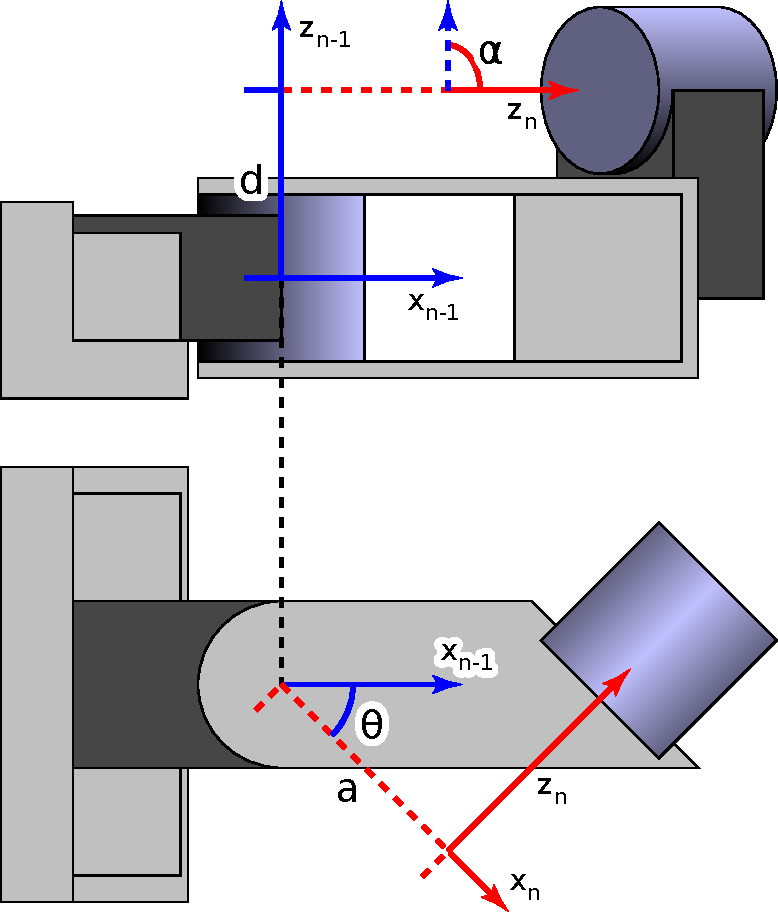
\includegraphics[height=.4\textheight]{Figures/Sample_Denavit-Hartenberg_Diagram.pdf}
 		\caption{Denavit-Hartenberg (DH) parameters: $a$, $\alpha$, $d$, and $\theta$~\cite{tekkotsu}}
 		\label{fig:DH}
	\end{center}
\end{figure}

Now, we can move from the base reference frame of some joint to the transformed reference frame of this joint using the transformation matrix $T_{DH}$, which consists of two translations and two rotations parametrized by the DH parameters of the joint:
\[T_{DH} = R_x(\alpha)T_x(a)R_z(\theta)T_z(d)\]
The analytical form of the resulting matrix from the above composition is the following:
\[
T_{DH} = 
\begin{bmatrix}
\cos\theta & -\sin\theta & 0 & a\\
\sin\theta\cos\alpha & \cos\theta\cos\alpha & -\sin\alpha & -d\sin\alpha\\
\sin\theta\cos\alpha & \cos\theta\sin\alpha & \cos\alpha & d\cos\alpha\\
0 & 0 & 0 & 1
\end{bmatrix}
\]
It is easy to see that the matrix above is an affine transformation matrix, because it is the product of affine transformation matrices.

\section{Mathematica}
Mathematica$^{\textrm{\copyright}}$ is a software tool for mathematical computations created by the Wolfram company (\url{www.wolfram.com}). This tool is widely-used, because, among other things, it can easily find solutions to differential equations and can perform symbolic computations. For the purposes of this thesis, we exploited its capability to perform large-scale symbolic computations with matrices and simplify symbolic expressions in reasonable time.

The following code excerpt is a small example of symbolic computation with Mathematica. We construct two matrices with cosines and sines containing two symbols, {\tt theta1} and {\tt theta2}. Next, we multiply those two matrices symbolically and finally we simplify the result:

\begin{small}
\begin{verbatim}
Matrix1 = {{Cos[theta1], -Sin[theta1]}, {Cos[theta1], -Cos[theta1]}};
Matrix2 = {{Cos[theta2], -Sin[theta2]}, {Cos[theta2], -Cos[theta2]}};
T = Matrix1.Matrix2;
Simplify[T];
MatrixForm[%]
\end{verbatim}
\end{small}

\noindent
The result of these symbolic computations is the following:
\begin{align*}
\text{Matrix1} &= \begin{bmatrix}
\cos\theta_1 & -\sin\theta_1\\
\cos\theta_1 & -\cos\theta_1
\end{bmatrix}\\
\text{Matrix2} &= \begin{bmatrix}
\cos\theta_2 & -\sin\theta_2\\
\cos\theta_2 & -\cos\theta_2
\end{bmatrix}\\
\text{T} &= \begin{bmatrix}
\cos\theta_1\cos\theta_2 - \cos\theta_2\sin\theta_1 &   \cos\theta_2 \sin\theta_1 - \cos\theta_1 \sin\theta_2\\
0 & \cos\theta_1 \cos\theta_2 - \cos\theta_1 \sin\theta_2
\end{bmatrix}\\
\text{T}_{\text{simplified}} &= \begin{bmatrix}
\cos\theta_2\left(\cos\theta_1 - \sin\theta_1\right) & \sin\left(\theta_1 - \theta_2\right)\\
 0 & \cos\theta_1 \left(\cos\theta_2 - \sin\theta_2\right)
\end{bmatrix}
\end{align*}
The example above is quite simple, but fully illustrates the symbolic capabilities of Mathematica and particularly the simplification step, which is very important for our work, given that we have to deal with much larger and more complex matrices.